\documentclass[]{report}

\usepackage{cmap}
\usepackage[russian]{babel}
\usepackage[utf8]{inputenc}
\usepackage[T2A]{fontenc}

\author{Егор Кузьмичев}
\title{Теоретико-игровой анализ транспортных пробок вокруг мест проведения массовых мероприятий}
%\contentsname{Содержание}

\begin{document}
\maketitle

ABSTRACT

\tableofcontents

\section{Введение}

\section{Место задачи в классификации теории игр}
В работе уделено внимание классификации теории игр, чтобы было понимание, какое место задача занимает в отрасли знания.

\subsection{Классификация теории игр}
%Выбор игрока влияет на других игроков.
%Кооперативная теория игр
%Некооперативная теория игр
%Игры в нормальной форме
%Доминантные и доминирующие стратегии
%Минимакс теорема
%Игры в развернутой форме
%Равновесие совершенное по подыграм
%Повторяющиеся игры
%Глобальные игры (Global games)
%Игры в стратегической форме


\section{Пример Пигу}

Задача напоминает пример Пигу, рассмотренный в книге \cite{nisan}.
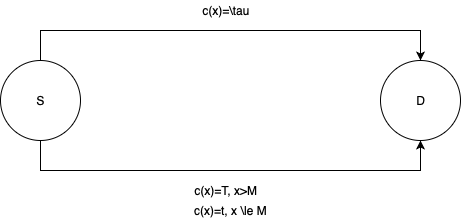
\includegraphics{img/pigou.png}


\section{Постановка задачи}

Существует $M$ парковочных мест

Издержки игроков $c(x)$:
 * $t$, если $\tilde N\le M$,
 * $T$, если $\tilde N>M$;
 * $\tau$, альтернативный маршрут,
 * $t<\tau<T$

$N$ игроков, $N >> M$.

$\tau$ — альтернативный маршрут. Сравнить его с лотереей ${t,T}$.

$P(t)$ задается $\tilde N$: $P=\frac{M}{\tilde{N}}$ (or $1$, if $M \le \tilde N$).

Чистое равновесие: $\frac{M}{\tilde N}t+(1-\frac{M}{\tilde{N}})T\approx\tau$.

-----------------

$\tilde{N}$ (количество севших за руль) : $\frac{M}{\tilde{N}}t+(1-\frac{M}{\tilde{N}})T\le\tau$.

${N-\tilde N}$ (кто едет транспортом) : $\frac{M}{(\tilde{N}+1)}t+(1-\frac{M}{\tilde{N}+1})T\ge\tau$.

-----------------

$T-\tau = \frac{M}{\tilde{N}}(T-t)$

$\tilde{N}=[\frac{M(T-t)}{T-\tau}]$ — pure equilibrium. Но «так не бывает», ибо неясно, кто эти счастливчики.

$p$ — вероятность сесть за руль.

$Q$[тебе достанется место] такова, что $\tau = Qt+(1-Q)T \Rightarrow Q(T-t)=T-\tau$, $Q*=\frac{T-\tau}{T-t}$.

Но! $Q$ должно быть вычислено как функция от $p$!

$(1-p)^{N-1} + \\ (N-1)p(1-p)^{N-2} + \\ C_{N-1}^2 p^2(1-p)^{N-2} + ... + \\ C_{N-1}^{M-1}p^{M-1}(1-p)^{N-M} + \\ C_{N-1}^{M}p^M(1-p)^{N-M-1}(\frac{M}{M+1}) + \\ C_{N-1}^{M+1}p^{M+1}(1-p)^{N-M-2}(\frac{M}{M+2}) + \\ p^{N-1}\frac{M}{N} = \\ Q^*$

Решить как обратную функцию, найти $p^*$ — решение $p^*(\frac{T-\tau}{T-t})$.

Гипотеза: в равновесии $Np^* >> M$.

\section{Место задачи в классификации теории игр}

\section{Актуальность задачи}

\section{Новизна задачи}



\end{document}
